\chapter{Stack}\label{chp:stack}

Stack data structure helps you get the last entered data in O(1) time.
In generally we proces arr[0..idx] elements and push them onto the stack.

\begin{marginfigure}  
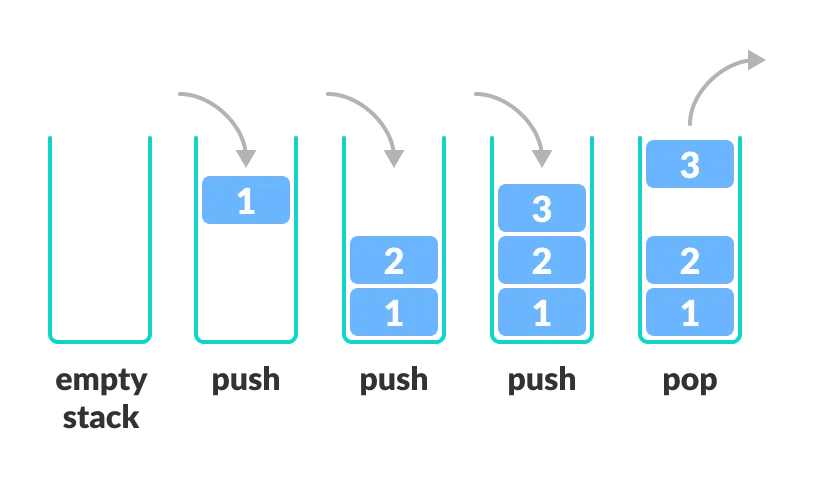
\includegraphics[width=\marginparwidth]{../resources/stack_intro.png}
\caption{stack in action}
\end{marginfigure}

The stack can keep the subsequence or the subarray, depending upon the pop strategy.

Stack is used when you want to have relative sorting of data w.r.t \verb|arr[idx]|

Problems to understand stack.
\begin{exercise}
    \begin{enumerate}
        \item Rain water harvesting.
        \item Palindromic Check, Longest Palindromic Length
        \item Valid Parenthesis, Longest Valid Parenthesis
        \item Next Greator Element (and related)
        \item all subarray sum(with constrain on max/min element of subarray) without caluclating all subarray. (i.e expected complexiy is linear)
    \end{enumerate}
\end{exercise}

% Pratice problem list
second next Greator
kth next Greator
Widard Strenght.

% TO-DO: Convert marginfigure to a environemtn acceptin g width & hegiht. use xparse package for flexible input

% Include Fils
% \import{./}{next-greator-element.tex} %use this version if you want include from subdirectory.

\begin{problem}{Next Greator Element}
    For a given arr[], find the next greater element for each element of the array in order of their appearance in the array.

    Example: arr[] = [6 8 0 1 3], sarr[] = [8 -1 1 3 -1].
    \footnotetext{gfg or LC496}
\end{problem}

\begin{solution}[Brute Force | $O(n^2)$]

    In the brute force , you will have two for loop and second loop will be depednet upon first for loop.

    \begin{code}
        //all of these are related and one can be 
        //easiely convertible to other.
        (a) for(int i=0;i<size;i++) 
            for(j=i;j<size;j++)

        (b) for(int i=0;i<size;i++)
            for(j=0;j>=0;j--)
        
        (c) for(int i=size-1;i>=0;i--)
            for(j=0;j<i;j++)
        
        (d) for(int i=size-1;i>=0;i--)
            for(int j=i;j<size;j++)
    \end{code}

    The above type of pattern has high chance(~as Aditya its 100\%) of applying stack to select the 2nd index j.
    \footnote{https://www.youtube.com/watch?v=P1bAPZg5uaE}

    \begin{code2}[Select One j for all i]
        vector<lli> firstGreator(vector<lli> arr)
        {
            int size = arr.size();
            vector<lli> ans(size,-1);
            
           for(int i=0;i<size;i++)
           {    
               for(int j=i+1;j<size;j++)
               {
                   if(arr[j] >arr[i])
                   {
                       ans[i] = arr[j];
                       break;
                   }
               }
           }
           
           return ans;
        }
    \end{code2}

\end{solution}

\begin{solution}[Stack | $O(n)$]
    We will maintain a monotonic decreasing stack.
   
    For a monotonic decreasing stack.\\
    \faHandPointRight\hspace{2mm}{we push array element to stack if current element is smaller than stack tidx}.\\
    \faHandPointRight\hspace{2mm}{we pop a element from stack if current element is greator than stack tidx.}
   
    You can understand this as, \rfl{we are maintaing a decreasing stack. we must be ensure that stack element at all time must be decreasing + we \textbf{must} push current element to stack.}

    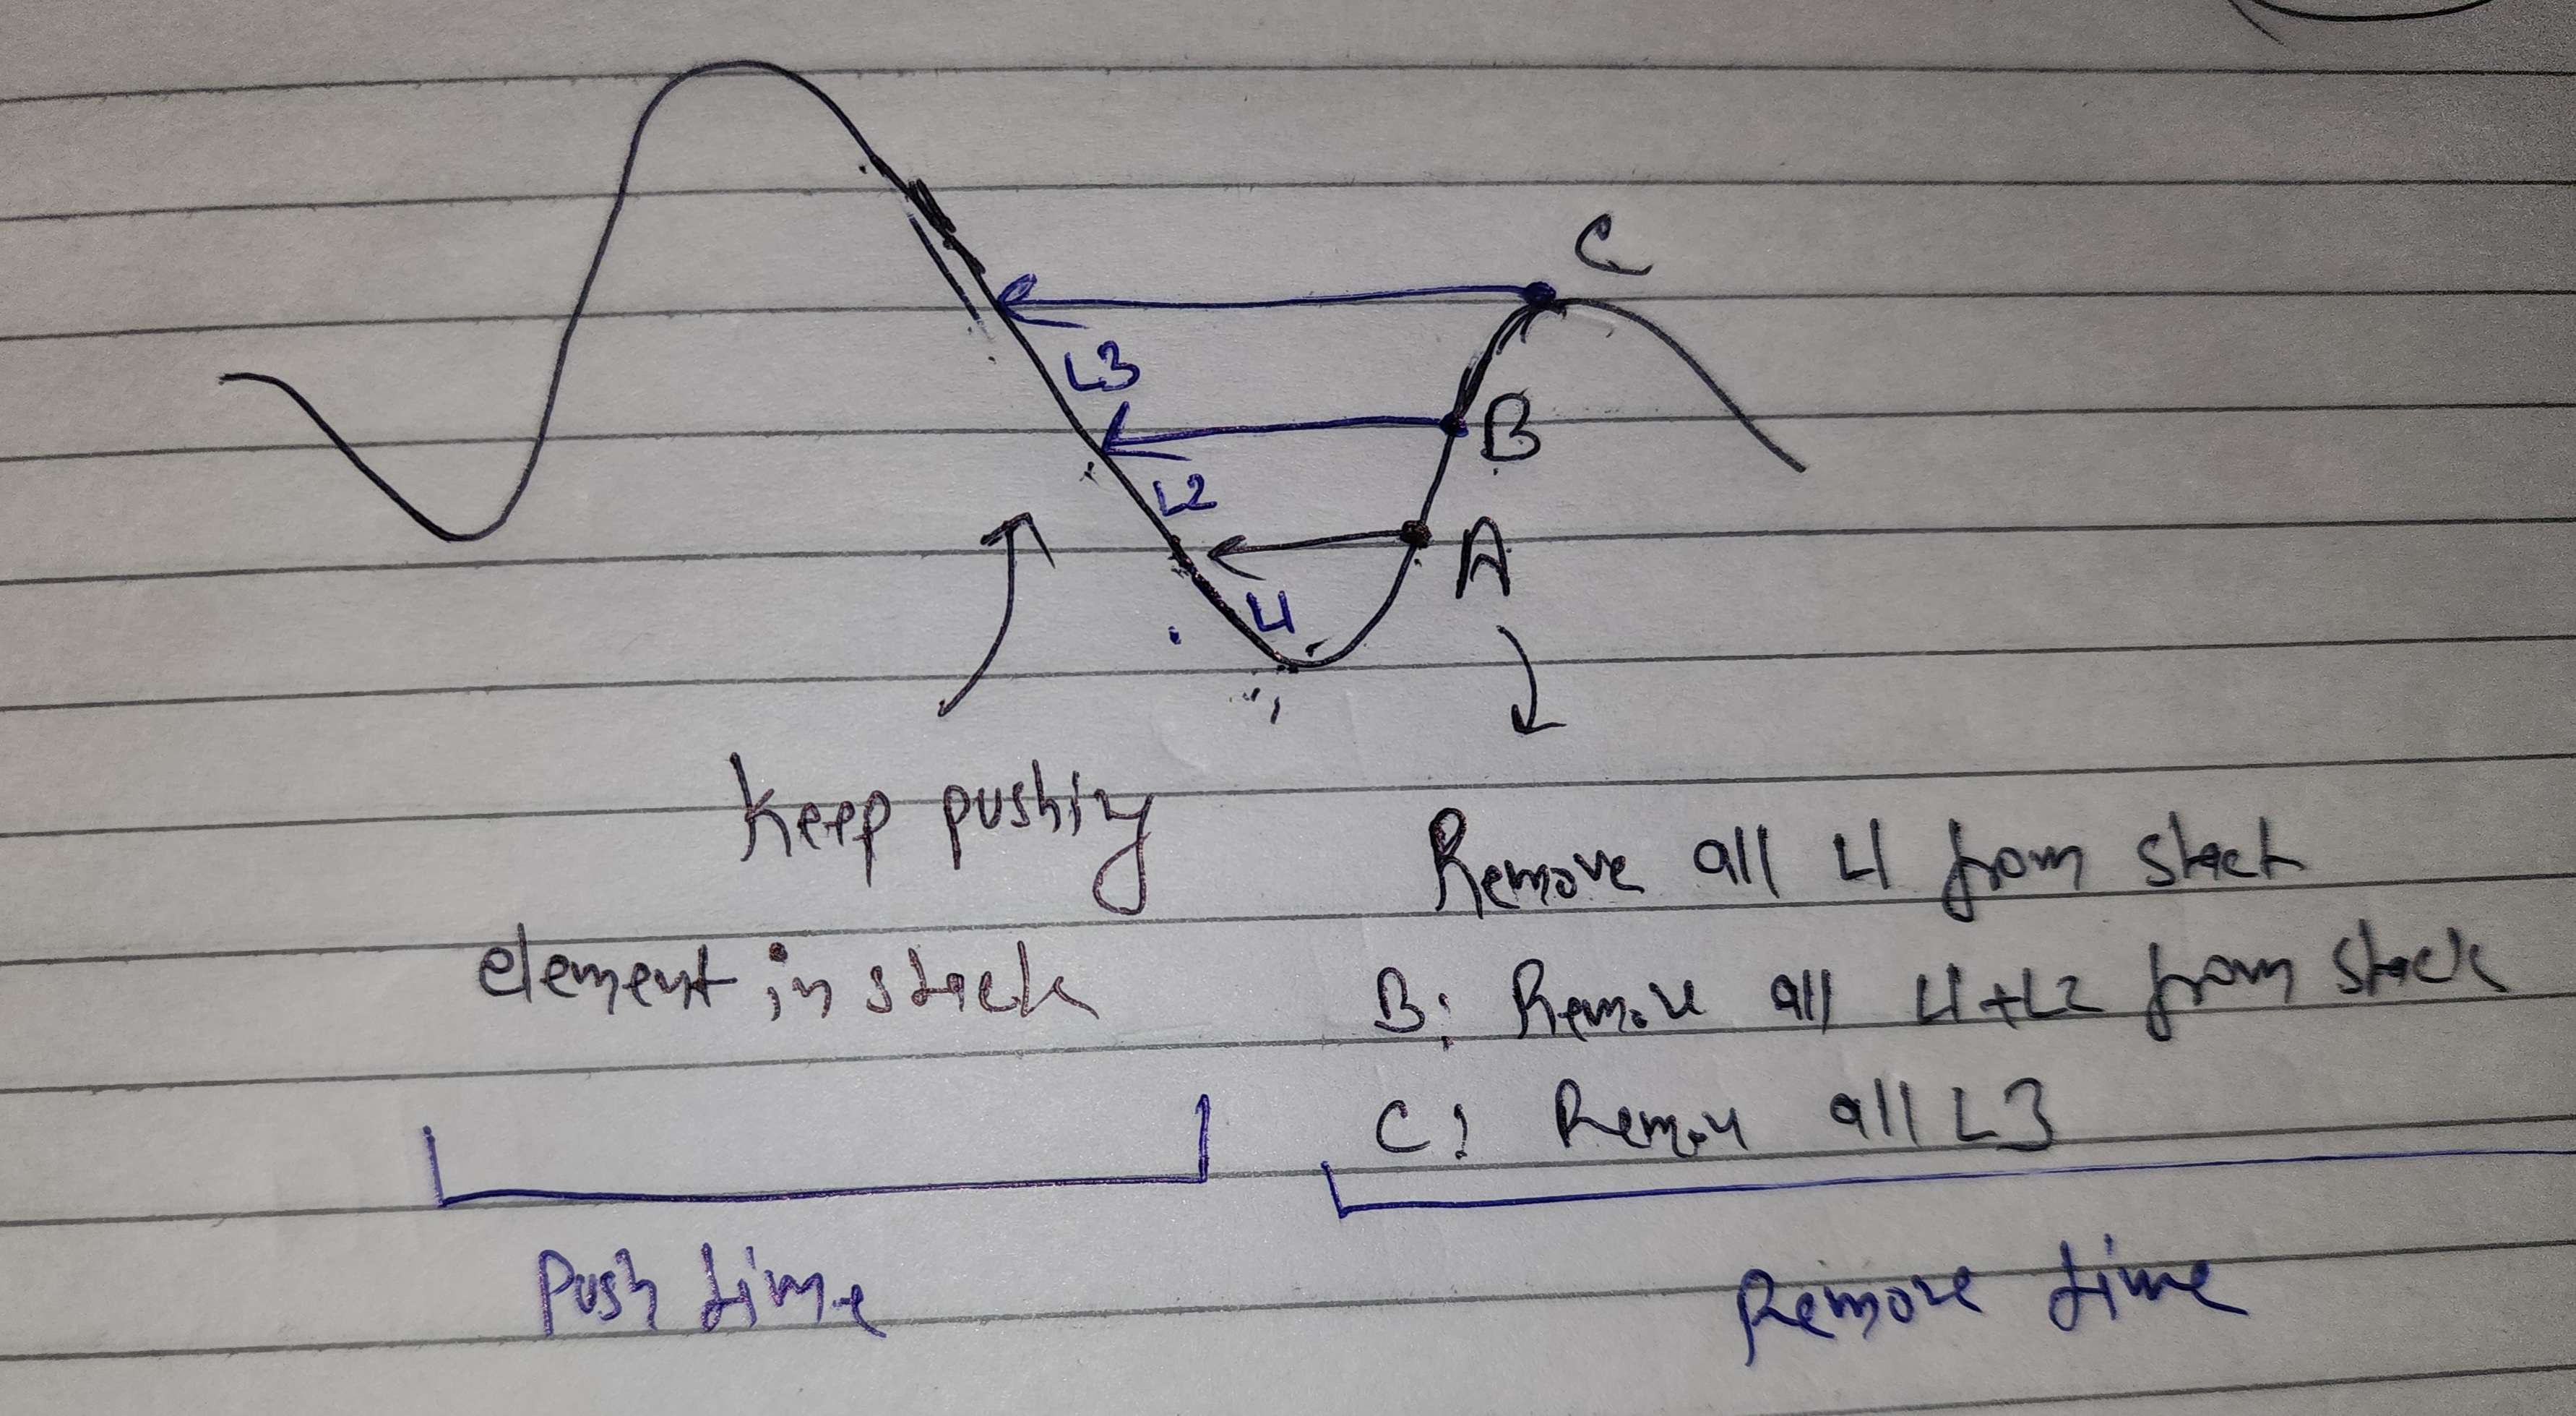
\includegraphics[width=0.7\textwidth]{./resources/monotonic-decreasing-stack.jpg}

    \begin{fullwidth}
    \begin{code3}[Reference Code]
        typedef long long int lli;
        #define tidx st.back()
        vector<lli> findGreatorStack(vector<lli> arr)
        {
            int size = arr.size();
            vector<lli> ans(size,-1);
            
            vector<int> st;  
            for(int i=0;i<size;i++)
            {
                //step(a):prepare stack for the insertion of arr[i]
                while(!st.empty() && arr[tidx]<arr[i])
                {
                    ans[tidx] = arr[i];
                    st.pop_back();
                }
                
                //step(b): insert
                st.push_back(i);
            }
            
            return ans;
        }

    /* few points to consider for above implemention*/
    (a) we have used vector in place of stack. (as printing st durign debugging will be easy this way)
    (b) we are pushing index to st, instead of index values.
    (c) the popping is same like incrementing l in two pointer. (we first ensure that l..r-1 is ready to accept r, then include r in range.)

    (d) How it is different from two pointer?
    (e) Can i say that st can have any subsequence depending upon the initial array? 

    /* places of interest*/
    There are 3 places where the knowledge of index tidx & i can be used.
    (a) Before popping. (nge problem series, ngarr[tidx]=i)
    (b) After popping. (rain water problem) (for element being popped. tidx is left_max, i is righ_max)
    (c) Before insertion.  (pge problem seris, pgarr[i] = tidx)

    \end{code3}
\end{fullwidth}
\lipsum[1-4]
\end{solution} % this will work too
\begin{problem}{Trapping Rain Water}
    Given n non-negative integers representing height of building in one-dimension. Assuming width of each building as 1unit. Compute how much water will be trapped by these building.

    \footnotetext{LC42}
\end{problem}

\begin{solution}[solution summary]
    There are various ways to solve this problem.

    \begin{guide}

        \item For current building, if you could find what is leftmost building which is just greator than arr[i] and what is rightmost building which is just greator then arr[i]. (i.e previousGreatorElement + nextGreatorElement).
        
        Then, water trapped by arr[i] would be \verb|min(pg,ng)-arr[i]|

        Try to use DP to calculate pgarr and ngarr.

        \item Can you use stack to find pg and ng for arr[i]?
        
        \item Can you try to use two-pointer?
    \end{guide}

\end{solution}

\begin{solution}[Stack | O(n)]
    Lets use stack to solve this problem.

    Recall
\end{solution}